After establishing a theoretical foundation both about multigrid methods and evolutionary grammar-based optimization techniques, the first primary goal of this thesis is to develop a formal language for expressing arbitrarily structured multigrid solvers in a generalized way.
For this purpose, first observe that the multigrid solvers described Section~\ref{sec:multigrid-cycles} can be all classified by their \emph{cycle type}.
Each such cycle possesses a distinct computational pattern which stems from the number of recursive descents performed on each level of the method.
For instance a V-cycle is characterized by exactly one recursive descent per level.
All these classically considered multigrid cycles employ a fixed uniform number of recursive descents and smoothing steps per discretization level, which is determined by the parameters $\gamma$, $\nu_1$ and $\nu_2$ in Algorithm~\ref{alg:multigrid-cycle}.
While the representation of a multigrid method as a recursive cycle yields a formally simple and easily parameterizable algorithmic formulation it also enforces unnecessary restrictions on its structure.
Consider for instance the multigrid method depicted in Figure~\ref{fig:non-traditional-multigrid-cycle}.
\begin{figure}
	\begin{subfigure}{0.1\textwidth}
		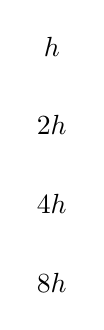
\begin{tikzpicture}
			\node   (h) at (-0.75, 4){$h$};
			\node   (2h) at (-0.75, 3){$2h$};
			\node   (4h) at (-0.75, 2){$4h$};
			\node   (8h) at (-0.75, 1){$8h$};
		\end{tikzpicture}
	\end{subfigure}
	\begin{subfigure}{0.9\textwidth}
		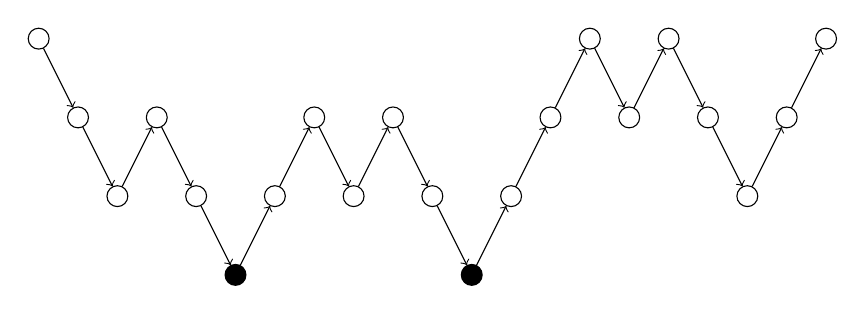
\begin{tikzpicture}
			\node	(a) at (0,4) [draw, circle,scale=0.8] {};
			\node	(b) at (0.5,3) [draw, circle,scale=0.8] {};
			\node	(c) at (1,2) [draw, circle,scale=0.8] {};
			\node	(d) at (1.5,3) [draw, circle, scale=0.8] {};
			\node	(e) at (2,2) [draw, circle, scale=0.8] {};
			\node	(f) at (2.5,1) [draw, circle,scale=0.8,fill=black] {};
			\node	(g) at (3,2) [draw, circle,scale=0.8] {};
			\node	(h) at (3.5,3) [draw, circle,scale=0.8] {};
			\node	(i) at (4,2) [draw, circle,scale=0.8] {};
			\node	(j) at (4.5,3) [draw, circle,scale=0.8] {};
			\node	(k) at (5,2) [draw, circle,scale=0.8] {};
			\node	(l) at (5.5,1) [draw, circle,scale=0.8,fill=black] {};
			\node	(m) at (6,2) [draw, circle,scale=0.8] {};
			\node	(n) at (6.5,3) [draw, circle,scale=0.8] {};
			\node	(o) at (7,4) [draw, circle,scale=0.8] {};
			\node	(p) at (7.5,3) [draw, circle,scale=0.8] {};
			\node	(q) at (8,4) [draw, circle,scale=0.8] {};
			\node	(r) at (8.5,3) [draw, circle,scale=0.8] {};
			\node	(s) at (9,2) [draw, circle,scale=0.8] {};
			\node	(t) at (9.5,3) [draw, circle,scale=0.8] {};
			\node	(u) at (10,4) [draw, circle,scale=0.8] {};
			\draw 
			(a) edge[->] (b) 
			(b) edge[->] (c)
			(c) edge[->] (d)
			(d) edge[->] (e)   
			(e) edge[->] (f)
			(f) edge[->] (g)
			(g) edge[->] (h)
			(h) edge[->] (i)
			(i) edge[->] (j)
			(j) edge[->] (k)
			(k) edge[->] (l)
			(l) edge[->] (m)
			(m) edge[->] (n)
			(n) edge[->] (o)
			(o) edge[->] (p)
			(p) edge[->] (q)
			(q) edge[->] (r)
			(r) edge[->] (s)
			(s) edge[->] (t)
			(t) edge[->] (u)
			;
		\end{tikzpicture}
	\end{subfigure}
	\caption{Example for a non-traditional multigrid method.}
	\label{fig:non-traditional-multigrid-cycle}
\end{figure}
While this method reaches the coarsest level twice and, hence, at first sight looks similar to a W-cycle, it employs a unique pattern of computations that is completely different from those of any of the traditional multigrid cycles.
As a consequence, this method can not be represented within the classical framework of multigrid cycles, as formulated in Algorithm~\ref{alg:multigrid-cycle}.
To overcome these limitations and construct multgrid methods with an arbitrary sequence of computations on each discretization level, as illustrated by the example in Figure~\ref{fig:non-traditional-multigrid-cycle}, a new formal language for their representation is needed.
The first step towards the development of this language is to find a way to represent the current state within each step of a multigrid method and then define transition rules between those states.
\section{Multigrid States and Transitions}
In order to determine how the state of a multigrid method can be represented, we need to reconsider our original formulation of a multigrid cycle in Algorithm~\ref{alg:multigrid-cycle}.
As it can be seen here, on each level $l > 0$ the following operations are employed within a multgrid cycle:
\begin{description}
	\item[Smoothing:] Reduce the oscillatory error components of the approximate solution $\tilde{\bm{x}}_h$ on the current level. 
	\begin{equation*}
		\tilde{\bm{x}}_h = \tilde{\bm{x}}_h + \omega M_h^{-1} \left( \bm{b}_h - A_h \tilde{\bm{x}}_h \right) \; \text{where} \; A_h = M_h + N_h
	\end{equation*}
	\item[Restriction:] Restrict the residual to obtain the right-hand side $\bm{b}_{2h}$ of the error equation on the next coarser level.
	\begin{align*}
		\tilde{\bm{x}}_{2h} & = 0 \\
 		\bm{b}_{2h} & = I_h^{2h} (\bm{b}_h - A_h \tilde{\bm {x}}_h)
	\end{align*}
	\item[Coarse-Grid Correction:] Prolongate a correction $\tilde{\bm{x}}_{2h}$ obtained on a coarser grid to reduce the low-frequency error components of the approximate solution $\tilde{\bm{x}}_h$.
	\begin{equation*}
		\tilde{\bm{x}}_h = \tilde{\bm{x}}_h + I_{2h}^h \tilde{\bm{x}}_{2h}
	\end{equation*}
\end{description}
Now note that except for the operators $A_h$, $I_h^{2h}$ and $I_{2h}^h$ the result of each of these operations exclusively depends on the current value of the approximate solution on subsequent levels, i.e. $\tilde{\bm{x}}_{h}$ and $\tilde{\bm{x}}_{2h}$, and the right-hand side $b_h$.
However, in contrast to coarse-grid correction which utilizes the current approximate solution on the coarse grid, both smoothing and restriction are based on computing the residual $\bm{r}_h = \bm{b}_h - A_h \tilde{\bm {x}}_h$ first, which can be considered as an intermediate step.
We can therefore distinguish these operations by considering whether the residual has been computed or not.
Therefore, the value of these variables uniquely identify the current state within each step of the method.
To illustrate this in a more concrete way, consider the sequence of operations shown in Algorithm~\ref{alg:example-three-grid-method}.
\begin{algorithm}
	\begin{algorithmic}[1]
		\State $\tilde{\bm{x}}_{h} = 0$
		\State $\bm{r}_{h} = \bm{b}_{h} - M_h \tilde{\bm{x}}_{h} $
		\State $\quad \tilde{\bm{x}}_{2h} = 0$
		\State $\quad \bm{b}_{2h} = I_{h}^{2h} r_{h}$
		\State $\quad \bm{r}_{2h} = \bm{b}_{2h} - M_{2h} \tilde{\bm{x}}_{2h}$
		\State $\quad \tilde{\bm{x}}_{2h} = \tilde{\bm{x}}_{2h} + I_{4h}^{2h} M_{4h}^{-1} I_{2h}^{4h} \bm{r}_{2h}$
		\State $\quad \bm{r}_{2h} = \bm{b}_{2h} - M_{2h} \tilde{\bm{x}}_{2h}$
		\State $\quad \tilde{\bm{x}}_{2h} = \tilde{\bm{x}}_{2h} + 0.6 \cdot D_{2h}^{-1} \bm{r}_{2h}$
		\State $\tilde{\bm{x}}_{h} = \tilde{\bm{x}}_{h}  + I_{2h}^h \tilde{\bm{x}}_{2h}$
	\end{algorithmic}
\caption{Example for a three-grid V-cycle}
\label{alg:example-three-grid-method}
\end{algorithm}



